\documentclass[12pt]{article}
\newcommand{\ReportShortTitle}{Báo cáo chung nhóm}
\usepackage[a4paper,top=2.1cm,bottom=2.2cm,left=2.6cm,right=2.2cm,headheight=15pt]{geometry}
\usepackage{fontspec}
\setmainfont{Times New Roman}
\setsansfont{Arial}
\setmonofont{Menlo}[Scale=0.86]
\usepackage{microtype}
\usepackage{setspace}
\setstretch{1.22}
\usepackage{parskip}
\setlength{\parindent}{1.1cm}
\setlength{\parskip}{3pt}

\usepackage{xcolor}
% Hệ màu đơn sắc: chỉ dùng đen, trắng và các mức xám để in ấn chuyên nghiệp.
\definecolor{Primary}{gray}{0}
\definecolor{Secondary}{gray}{0}
\definecolor{Accent}{gray}{0.72}
\definecolor{SoftBlue}{gray}{0.94}
\definecolor{SoftGray}{gray}{0.97}
\definecolor{Success}{gray}{0}
\definecolor{Warning}{gray}{0}
% Màu chỉ dùng bên trong khối mã nguồn.
\definecolor{CodeKeyword}{HTML}{1F4E79}
\definecolor{CodeComment}{HTML}{3F6B45}
\definecolor{CodeString}{HTML}{8A4B08}

\usepackage{graphicx}
\usepackage{booktabs}
\usepackage{longtable}
\usepackage{tabularx}
\usepackage{array}
\usepackage{makecell}
\usepackage{multirow}
\usepackage{enumitem}
\usepackage{amsmath,amssymb}
\usepackage{tikz}
\usetikzlibrary{arrows.meta,positioning,shapes.geometric,fit}
\usepackage[most]{tcolorbox}
\usepackage{listings}
\usepackage{needspace}
\renewcommand{\lstlistingname}{Đoạn mã}
\renewcommand{\lstlistlistingname}{Danh sách đoạn mã}
\renewcommand{\contentsname}{MỤC LỤC}
\usepackage{titlesec}
\usepackage{fancyhdr}
\usepackage{lastpage}
\usepackage{hyperref}
\hypersetup{colorlinks=true,linkcolor=Primary,urlcolor=Secondary,citecolor=Primary,pdfborder={0 0 0}}

\setlist[itemize]{leftmargin=1.2cm,itemsep=2pt,topsep=3pt}
\setlist[enumerate]{leftmargin=1.2cm,itemsep=2pt,topsep=3pt}
\renewcommand{\arraystretch}{1.25}
\newcolumntype{Y}{>{\raggedright\arraybackslash}X}
\newcolumntype{C}[1]{>{\centering\arraybackslash}p{#1}}
\newcolumntype{L}[1]{>{\raggedright\arraybackslash}p{#1}}

\titleformat{\section}{\Large\bfseries\color{Primary}}{\thesection.}{0.55em}{}
\titleformat{\subsection}{\large\bfseries\color{Secondary}}{\thesubsection.}{0.5em}{}
\titleformat{\subsubsection}{\normalsize\bfseries\color{Primary}}{\thesubsubsection.}{0.5em}{}
\titlespacing*{\section}{0pt}{16pt}{7pt}
\titlespacing*{\subsection}{0pt}{11pt}{5pt}

\pagestyle{fancy}
\fancyhf{}
\fancyhead[L]{\small\color{Primary}\textbf{ĐỒ ÁN ESP32-S3}}
\fancyhead[R]{\small\color{Secondary}\ReportShortTitle}
\fancyfoot[L]{\small Nhóm 3 thành viên}
\fancyfoot[R]{\small Trang \thepage/\pageref{LastPage}}
\renewcommand{\headrulewidth}{0.5pt}
\renewcommand{\footrulewidth}{0.4pt}

\newtcolorbox{summarybox}[1][Tóm tắt]{
  enhanced, breakable, colback=SoftBlue, colframe=Secondary,
  title=\textbf{#1}, coltitle=white, colbacktitle=Secondary,
  boxrule=0.7pt, arc=2mm, left=3mm, right=3mm, top=2mm, bottom=2mm
}
\newtcolorbox{evidencebox}[1][Minh chứng]{
  enhanced, breakable, colback=SoftGray, colframe=Primary,
  title=\textbf{#1}, coltitle=white, colbacktitle=Primary,
  boxrule=0.6pt, arc=1.5mm, left=3mm, right=3mm, top=2mm, bottom=2mm
}
\newtcolorbox{warningbox}[1][Lưu ý]{
  enhanced, breakable, colback=Accent!12, colframe=Warning,
  title=\textbf{#1}, coltitle=white, colbacktitle=Warning,
  boxrule=0.6pt, arc=1.5mm, left=3mm, right=3mm, top=2mm, bottom=2mm
}

\lstdefinestyle{firmware}{
  language=C++,
  basicstyle=\ttfamily\fontsize{8.35}{10.2}\selectfont,
  keywordstyle=\color{CodeKeyword}\bfseries,
  commentstyle=\color{CodeComment}\itshape,
  stringstyle=\color{CodeString},
  numbers=left,
  numberstyle=\sffamily\fontsize{6.8}{8.2}\selectfont\color{black!48},
  numbersep=9pt,
  frame=lines,
  framerule=0.45pt,
  rulecolor=\color{black!68},
  backgroundcolor=\color{white},
  framesep=5.5pt,
  breaklines=true,
  breakatwhitespace=false,
  breakindent=1.25em,
  columns=fullflexible,
  keepspaces=true,
  showstringspaces=false,
  tabsize=2,
  escapeinside={(*@}{@*)},
  xleftmargin=1.1em,
  xrightmargin=0.25em,
  framexleftmargin=1.0em,
  framexrightmargin=0.45em,
  aboveskip=9pt,
  belowskip=10pt,
  abovecaptionskip=6pt,
  belowcaptionskip=0pt,
  captionpos=b
}

% Chú thích tiếng Việt được render bằng XeLaTeX ngay trong khung mã.
\newcommand{\VNCodeComment}[1]{%
  \parbox[t]{0.93\linewidth}{%
    \raggedright\color{CodeComment}\sffamily\fontsize{7.7}{9.1}\selectfont\itshape
    \textcolor{CodeComment}{\textbf{//}}\enspace #1}%
}

\newcommand{\ProjectTitle}{THIẾT BỊ ĐEO THEO DÕI SỨC KHỎE, PHÁT HIỆN TÉ NGÃ VÀ ĐỊNH VỊ DÙNG ESP32-S3}
\newcommand{\GroupMembers}{Phạm Hùng Tiến -- Hồ Sĩ Phú -- Quách Gia Thịnh}
\newcommand{\ReportDate}{Tháng 8 năm 2026}
\newcommand{\RepositoryURL}{https://github.com/PhamHungTien/esp32-s3-health-monitor}
\newcommand{\RepositoryDisplay}{github.com/PhamHungTien/esp32-s3-health-monitor}
\newcommand{\UniversityName}{TRƯỜNG ĐẠI HỌC KHOA HỌC TỰ NHIÊN}
\newcommand{\UniversitySystem}{ĐẠI HỌC QUỐC GIA THÀNH PHỐ HỒ CHÍ MINH}
\newcommand{\FacultyName}{KHOA ĐIỆN TỬ -- VIỄN THÔNG}

\newcommand{\CoverInstitution}{%
  \centering
  
\includegraphics[height=2.8cm]{assets/branding/hcmus_logo_user.png}\par
  \vspace{0.2cm}
  {\sffamily\bfseries\small\color{Primary}\UniversitySystem\par}
  \vspace{2pt}
  {\sffamily\bfseries\fontsize{16}{20}\selectfont\color{Primary}\UniversityName\par}
  \vspace{3pt}
  {\sffamily\bfseries\large\color{Secondary}\FacultyName\par}
  \vspace{0.35cm}
  {\color{Primary}\rule{0.84\textwidth}{1.0pt}\par}
}

\newcommand{\CoverBands}{%
  \begin{tikzpicture}[remember picture,overlay]
    \fill[Primary] (current page.north west) rectangle ([yshift=-4.5mm]current page.north east);
    \fill[Secondary] (current page.south west) rectangle ([yshift=3mm]current page.south east);
  \end{tikzpicture}%
}

\newcommand{\CoverField}[2]{%
  \noindent
  \begin{minipage}[t]{0.35\linewidth}
    \raggedright\strut\sffamily\bfseries\color{Primary}#1
  \end{minipage}\hfill
  \begin{minipage}[t]{0.61\linewidth}
    \raggedright\strut\sffamily\color{black}#2
  \end{minipage}\par
}

\hypersetup{
  pdftitle={\ProjectTitle\space -- \ReportShortTitle},
  pdfauthor={\GroupMembers},
  pdfsubject={Báo cáo đồ án thiết bị theo dõi sức khỏe dùng ESP32-S3},
  pdfkeywords={ESP32-S3, MAX30102, OLED, IMU, GPS, nhịp tim, SpO2, té ngã}
}

\newcommand{\MakeReportCover}[4]{%
  \hypersetup{pageanchor=false}
  \begin{titlepage}
    \thispagestyle{empty}
    \centering
    \CoverBands
    \vspace*{0.05cm}
    \CoverInstitution
    \vspace{0.45cm}
    {\sffamily\bfseries\normalsize\color{Secondary} BÁO CÁO ĐỒ ÁN\par}
    \vspace{0.35cm}
    {\sffamily\bfseries\fontsize{18}{23}\selectfont\color{Primary}\ProjectTitle\par}
    \vspace{0.6cm}
    \begin{tcolorbox}[width=0.84\textwidth,colback=SoftBlue,colframe=Secondary,arc=1.8mm,boxrule=0.8pt,left=4mm,right=4mm,top=2.7mm,bottom=2.7mm]
      \centering{\sffamily\bfseries\normalsize\color{Secondary} #1\par}
    \end{tcolorbox}
    \vfill
    \begin{tcolorbox}[width=0.84\textwidth,colback=white,colframe=Primary!48,arc=1.2mm,boxrule=0.6pt,left=6mm,right=6mm,top=4.5mm,bottom=4.5mm]
      \raggedright
      \CoverField{Người thực hiện}{#2}
      \vspace{2.1mm}
      \CoverField{Mã số sinh viên}{#3}
      \vspace{2.1mm}
      \CoverField{Nhóm}{03 thành viên}
      \vspace{2.1mm}
      \CoverField{Phạm vi báo cáo}{#4}
    \end{tcolorbox}
    \vfill
    {\sffamily\footnotesize\color{Secondary}\GroupMembers\par}
    \vspace{0.2cm}
    {\sffamily\footnotesize\color{Primary}\textbf{Mã nguồn đồ án: }
      \href{\RepositoryURL}{\RepositoryDisplay}\par}
    \vspace{0.2cm}
    {\sffamily\bfseries\small\color{Primary}Thành phố Hồ Chí Minh, \ReportDate\par}
    \vspace{0.2cm}
  \end{titlepage}
  \hypersetup{pageanchor=true}
  \clearpage
}

\newcommand{\MakeGroupCover}[1]{%
  \hypersetup{pageanchor=false}
    \begin{titlepage}
    \thispagestyle{empty}
    \centering
    \CoverBands
    \vspace*{0.05cm}
    \CoverInstitution
    \vspace{0.45cm}
    {\sffamily\bfseries\normalsize\color{Secondary} BÁO CÁO ĐỒ ÁN\par}
    \vspace{0.35cm}
    {\sffamily\bfseries\fontsize{18}{23}\selectfont\color{Primary}\ProjectTitle\par}
    \vspace{0.6cm}
    \begin{tcolorbox}[width=0.84\textwidth,colback=SoftBlue,colframe=Secondary,arc=1.8mm,boxrule=0.8pt,left=4mm,right=4mm,top=2.7mm,bottom=2.7mm]
      \centering{\sffamily\bfseries\normalsize\color{Secondary} #1\par}
    \end{tcolorbox}
    \vfill
    \begin{tcolorbox}[width=0.84\textwidth,colback=white,colframe=Primary!48,arc=1.2mm,boxrule=0.6pt,left=6mm,right=6mm,top=4.5mm,bottom=4.5mm]
      \sffamily
      {\bfseries\color{Primary}THÀNH VIÊN THỰC HIỆN\par}
      \vspace{3mm}
      \begin{tabularx}{\linewidth}{C{1.1cm} Y C{3.0cm}}
        \toprule
        \textbf{STT} & \textbf{Họ và tên} & \textbf{MSSV}\\
        \midrule
        1 & Phạm Hùng Tiến & 24207043\\
        2 & Hồ Sĩ Phú & 24207101\\
        3 & Quách Gia Thịnh & 24207105\\
        \bottomrule
      \end{tabularx}
    \end{tcolorbox}
    \vfill
    {\sffamily\footnotesize\color{Primary}\textbf{Mã nguồn đồ án: }
      \href{\RepositoryURL}{\RepositoryDisplay}\par}
    \vspace{0.2cm}
    {\sffamily\bfseries\small\color{Primary}Thành phố Hồ Chí Minh, \ReportDate\par}
    \vspace{0.2cm}
  \end{titlepage}
  \hypersetup{pageanchor=true}
  \clearpage
}

\newcommand{\Code}[1]{\texttt{#1}}
\newcommand{\OK}{\textcolor{Success}{\textbf{Đạt}}}
\newcommand{\Implemented}{\textcolor{Secondary}{\textbf{Đã cài đặt}}}
\newcommand{\NeedTest}{\textcolor{Warning}{\textbf{Cần thử thêm}}}
\newcommand{\Pending}{\textcolor{Warning}{\textbf{Cần hiệu chuẩn}}}


\begin{document}
\MakeGroupCover{BÁO CÁO CHUNG TỔNG KẾT NHÓM}

\tableofcontents
\clearpage

\section{Tóm tắt đồ án}

Nhóm xây dựng thiết bị nguyên mẫu dùng ESP32-S3 để đo nhịp tim, ước lượng nồng độ oxy trong máu, đếm bước, hiển thị trên OLED, phát hiện té ngã, lấy vị trí GPS và cung cấp dashboard qua Wi-Fi cục bộ. Chương trình chỉ dùng thành phần thuộc ESP32 Arduino Core; driver cảm biến, xử lý tín hiệu, parser và giao diện web được viết trong mã nguồn của nhóm.

\begin{summarybox}[Kết quả chính]
Ba thiết bị I2C được nhận đồng thời; OLED và dashboard hiển thị dữ liệu sức khỏe; MAX30102 phát hiện ngón tay và BPM hội tụ; IMU trả gia tốc nghỉ xấp xỉ 1$g$; GPS bắt FIX với 4 vệ tinh ở lần chạy cuối. ESP32-S3 phát mạng \Code{health-monitor}, phục vụ giao diện tại 192.168.4.1 và API JSON cập nhật mỗi 0,25 giây. Kênh LEDC cho buzzer và hai thao tác web đặt lại bước/hủy cảnh báo đã được cài đặt. Đếm bước, SpO$_2$ và té ngã vẫn cần thêm hiệu chuẩn hoặc phép thử thực tế.
\end{summarybox}

\section{Đối chiếu yêu cầu nộp bài}

Phần cuối buổi học ngày 23/07 nêu ba loại hồ sơ và yêu cầu phần việc cá nhân không trùng nhau. Nhóm chuẩn bị các tệp theo bảng sau.

\noindent\begin{tabularx}{\textwidth}{L{4.0cm} Y C{2.2cm}}
\toprule
\textbf{Hồ sơ/yêu cầu} & \textbf{Cách thực hiện} & \textbf{Đối chiếu}\\
\midrule
Bảng phân công và đánh giá & Một tệp chung, nêu tính năng, kết quả và tỷ lệ đóng góp của từng người & \OK\\
Báo cáo công việc cá nhân & Ba tệp riêng; mỗi tệp mô tả phần mã, phép thử và hạn chế của đúng mô-đun được giao & \OK\\
Báo cáo chung tổng kết & Một tệp dùng chung, tổng hợp kiến trúc, kết quả và phần chưa hoàn thiện & \OK\\
Không tính ``tìm tài liệu'' là nhiệm vụ & Mỗi thành viên chịu một khối kỹ thuật có đầu ra chạy được; tài liệu chỉ nằm ở mục tham khảo & \OK\\
Không trùng phần việc cá nhân & Tích hợp/hiển thị; PPG; IMU--GPS được tách thành ba phạm vi khác nhau & \OK\\
Báo cáo đúng tiến độ thực tế & SpO$_2$, đếm bước và té ngã được ghi rõ phần còn phải hiệu chuẩn/thử thêm & \OK\\
\bottomrule
\end{tabularx}

\section{Yêu cầu và phạm vi}

\begin{tabularx}{\textwidth}{L{4.4cm} Y C{2.1cm}}
\toprule
\textbf{Yêu cầu} & \textbf{Cách đáp ứng} & \textbf{Trạng thái}\\
\midrule
Đo nhịp tim & Thu PPG IR 100 Hz, dò nhịp, làm mượt BPM & \OK\\
Ước lượng SpO$_2$ & Ratio-of-ratios từ RED/IR, cờ chất lượng & \Pending\\
Phản hồi nhanh & BPM sau RR hợp lệ đầu tiên; SpO$_2$ dùng cửa sổ 64 mẫu & \OK\\
Đếm bước & Lọc gia tốc động, kiểm tra chu kỳ bước & \Implemented\\
Hiển thị tại chỗ & Driver SSD1306, BPM/SpO$_2$ cỡ lớn & \OK\\
Hiển thị trên web & Wi-Fi AP, captive portal, API JSON và dashboard responsive & \Implemented\\
Cảnh báo té ngã & Chuỗi rơi tự do--va đập--bất động & \Implemented\\
Định vị & UART, checksum NMEA, parser GGA/RMC & \OK\\
Âm báo & PWM LEDC trên GPIO42, hai âm xen kẽ khi ALERT & \Implemented\\
Không dùng thư viện ngoài & Driver và parser viết trong sketch & \OK\\
\bottomrule
\end{tabularx}

\section{Kiến trúc hệ thống}

\begin{figure}[htbp]
\centering
\begin{tikzpicture}[
  node distance=8mm and 12mm,
  block/.style={draw=black,rounded corners=1mm,fill=gray!7,minimum width=31mm,minimum height=11mm,align=center,font=\small},
  core/.style={draw=black,very thick,rounded corners=1mm,fill=gray!18,minimum width=40mm,minimum height=16mm,align=center,font=\bfseries},
  arrow/.style={-{Latex[length=2.2mm]},thick,color=black}
]
\node[core] (esp) {ESP32-S3 N16R8\\Bộ lập lịch không chặn};
\node[block,above left=of esp] (ppg) {MAX30102\\RED/IR, FIFO};
\node[block,left=of esp] (imu) {IMU 0x68\\Gia tốc, số bước};
\node[block,below left=of esp] (gps) {GPS UART\\NMEA 9600 baud};
\node[block,above right=of esp] (algo) {BPM, SpO$_2$\\Chất lượng tín hiệu};
\node[block,right=of esp] (fall) {Máy trạng thái\\phát hiện té ngã};
\node[block,below right=of esp] (oled) {OLED SSD1306\\Giao diện/cảnh báo};
\node[block,below=of esp] (web) {Wi-Fi AP + HTTP/DNS tự viết\\Dashboard và JSON API};
\draw[arrow] (ppg) -- (esp);
\draw[arrow] (imu) -- (esp);
\draw[arrow] (gps) -- (esp);
\draw[arrow] (esp) -- (algo);
\draw[arrow] (esp) -- (fall);
\draw[arrow] (esp) -- (oled);
\draw[arrow] (esp) -- (web);
\end{tikzpicture}
\caption{Sơ đồ khối kiến trúc tổng thể của thiết bị.}
\label{fig:block-architecture}
\end{figure}

\subsection{Bảng kết nối}

\begin{tabularx}{\textwidth}{L{3.4cm} L{3.0cm} L{3.0cm} Y}
\toprule
\textbf{Khối} & \textbf{Giao tiếp} & \textbf{Tài nguyên} & \textbf{Ghi chú}\\
\midrule
OLED SSD1306 & I2C, 0x3C & SDA GPIO8, SCL GPIO9 & VCC 3,3 V; GND chung\\
MAX30102 & I2C, 0x57 & Chung SDA/SCL & VCC 3,3 V; FIFO 100 Hz\\
IMU tương thích MPU & I2C, 0x68 & Chung SDA/SCL & WHO\_AM\_I 0x74; đọc gia tốc từ 0x3B\\
GPS & UART1 phần cứng & RX GPIO21, TX GPIO47 & GPS TX nối GPIO21; GPS RX nối GPIO47; 9600 baud\\
Loa piezo/buzzer & PWM LEDC & SPK+ GPIO42, SPK- GND & Cảnh báo té ngã; camera không dùng\\
USB & USB native & USB-Serial/JTAG & Nạp và nhật ký\\
Dashboard web & Wi-Fi 2,4 GHz & AP 192.168.4.1 & SSID \Code{health-monitor}; mật khẩu \Code{99999999}\\
\bottomrule
\end{tabularx}

\begin{warningbox}[Ràng buộc bo camera]
GPIO8 và GPIO9 cũng thuộc nhóm tín hiệu camera trên bo Freenove ESP32-S3 Camera. Trong cấu hình đồ án, camera không được sử dụng và phải tách khỏi hai chân này để tránh tranh chấp với bus I2C.
\end{warningbox}

\subsection{Hình ảnh các linh kiện chính}

\begin{figure}[htbp]
  \centering
  \begin{minipage}[t]{0.48\textwidth}
    \centering
    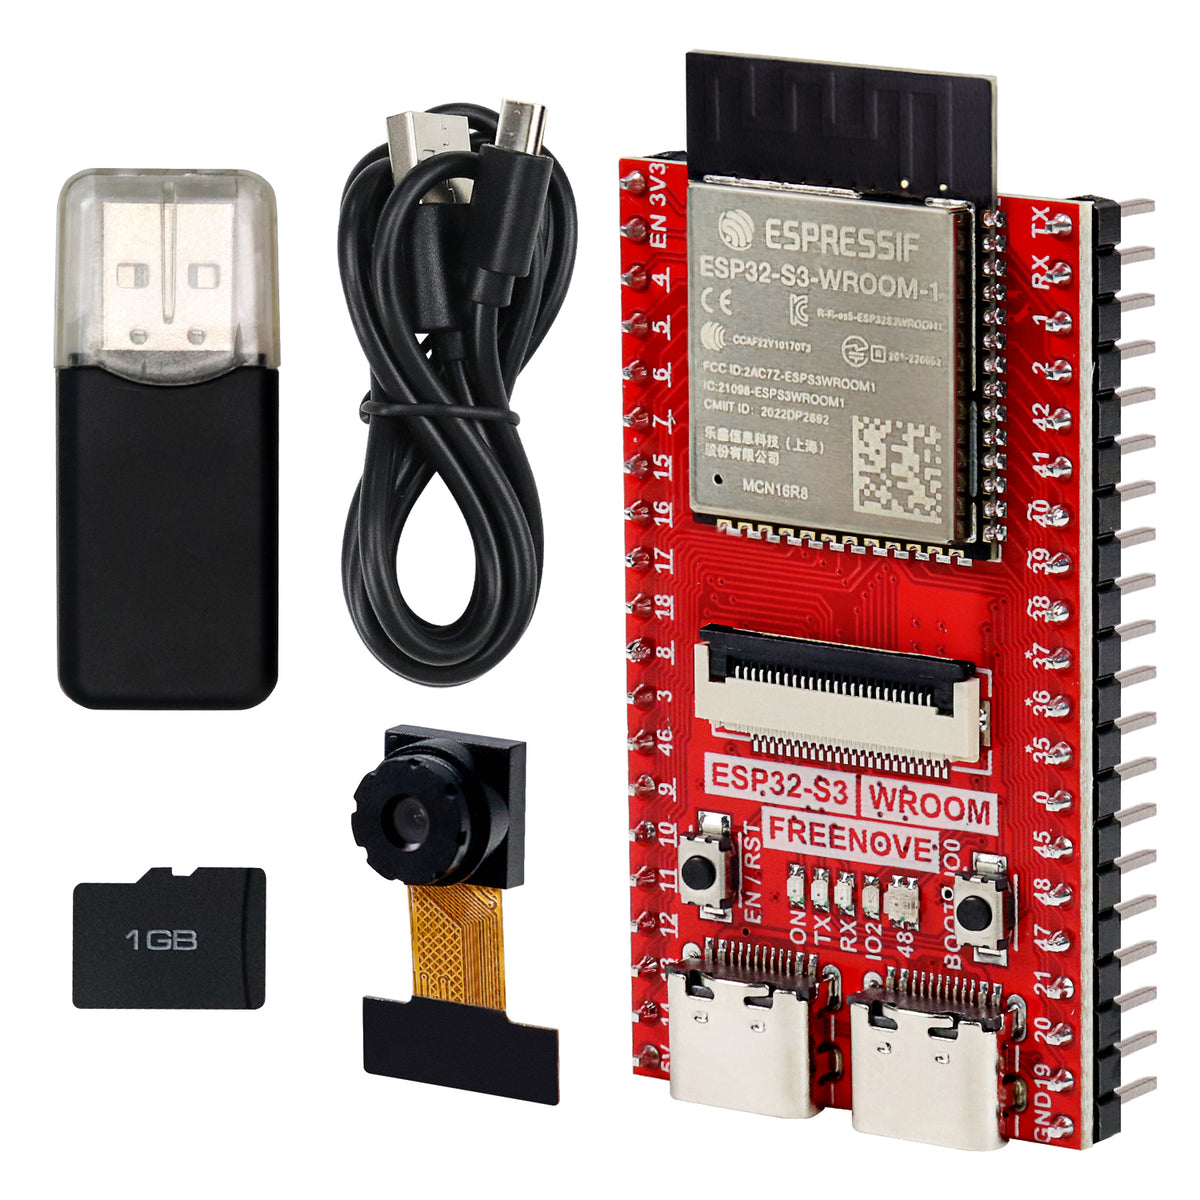
\includegraphics[width=0.88\linewidth,height=4.5cm,keepaspectratio]{assets/components/esp32s3_freenove.jpg}
    \\[2pt]\small (a) Bo điều khiển Freenove ESP32-S3 N16R8.
  \end{minipage}\hfill
  \begin{minipage}[t]{0.48\textwidth}
    \centering
    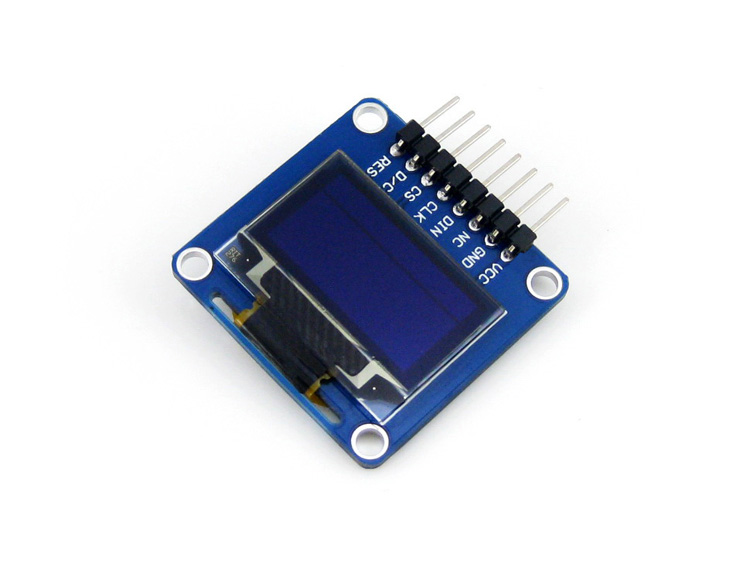
\includegraphics[width=0.88\linewidth,height=4.5cm,keepaspectratio,trim=110 30 110 30,clip]{assets/components/oled_ssd1306.jpg}
    \\[2pt]\small (b) OLED SSD1306 128x64 tham chiếu.
  \end{minipage}

  \vspace{5mm}
  \begin{minipage}[t]{0.48\textwidth}
    \centering
    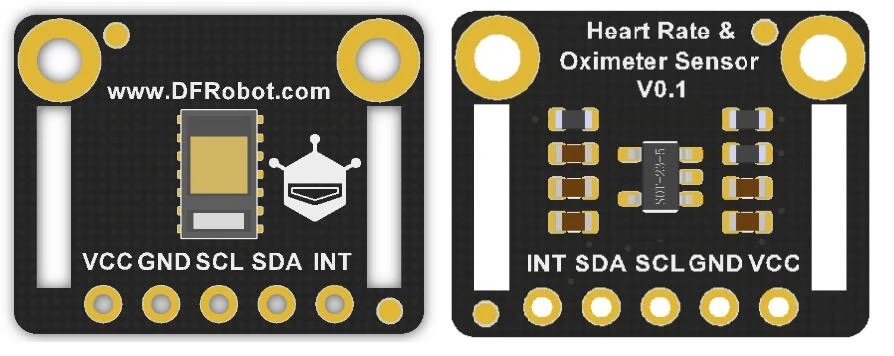
\includegraphics[width=0.90\linewidth,height=4.0cm,keepaspectratio]{assets/components/max30102_board_overview.jpg}
    \\[2pt]\small (c) Bo breakout MAX30102 tham chiếu.
  \end{minipage}\hfill
  \begin{minipage}[t]{0.48\textwidth}
    \centering
    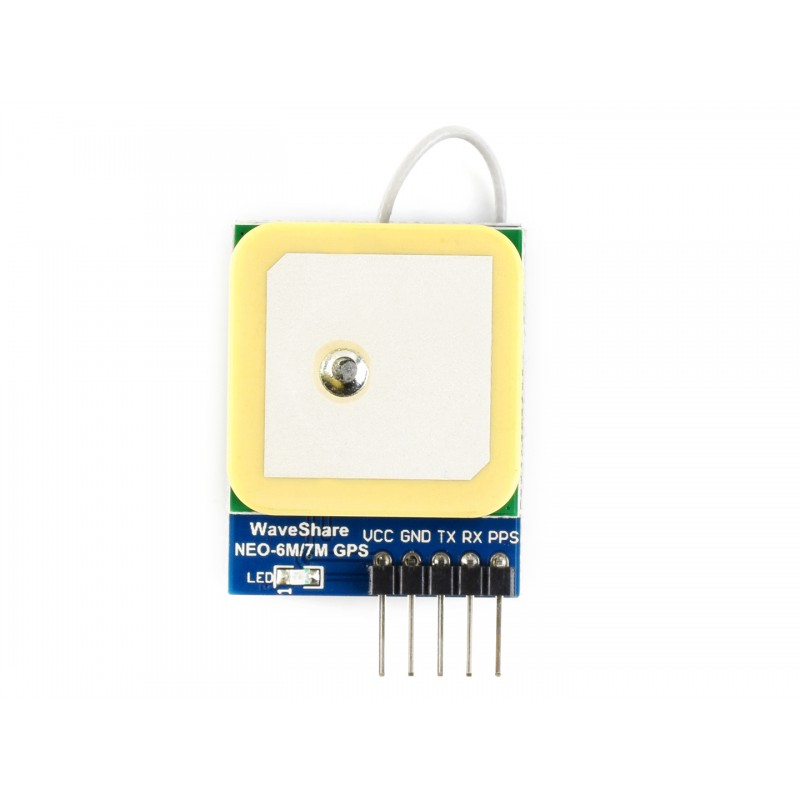
\includegraphics[width=0.66\linewidth,height=4.0cm,keepaspectratio,trim=180 55 180 55,clip]{assets/components/gps_neo6m_reference.jpg}
    \\[2pt]\small (d) Mô-đun GPS UART tham chiếu.
  \end{minipage}
  \caption{Nhóm linh kiện chính của nguyên mẫu. Ảnh bo điều khiển là đúng dòng sản phẩm; ảnh OLED, MAX30102 và GPS thể hiện loại linh kiện/giao tiếp, không dùng để khẳng định nhà sản xuất của các bo breakout đang lắp. Nguồn: Freenove, Waveshare và DFRobot.}
  \label{fig:group-components}
\end{figure}

\Needspace{0.62\textheight}
\subsection{Nguyên mẫu hoạt động trên mạch thử}

\begin{figure}[htbp]
  \centering
  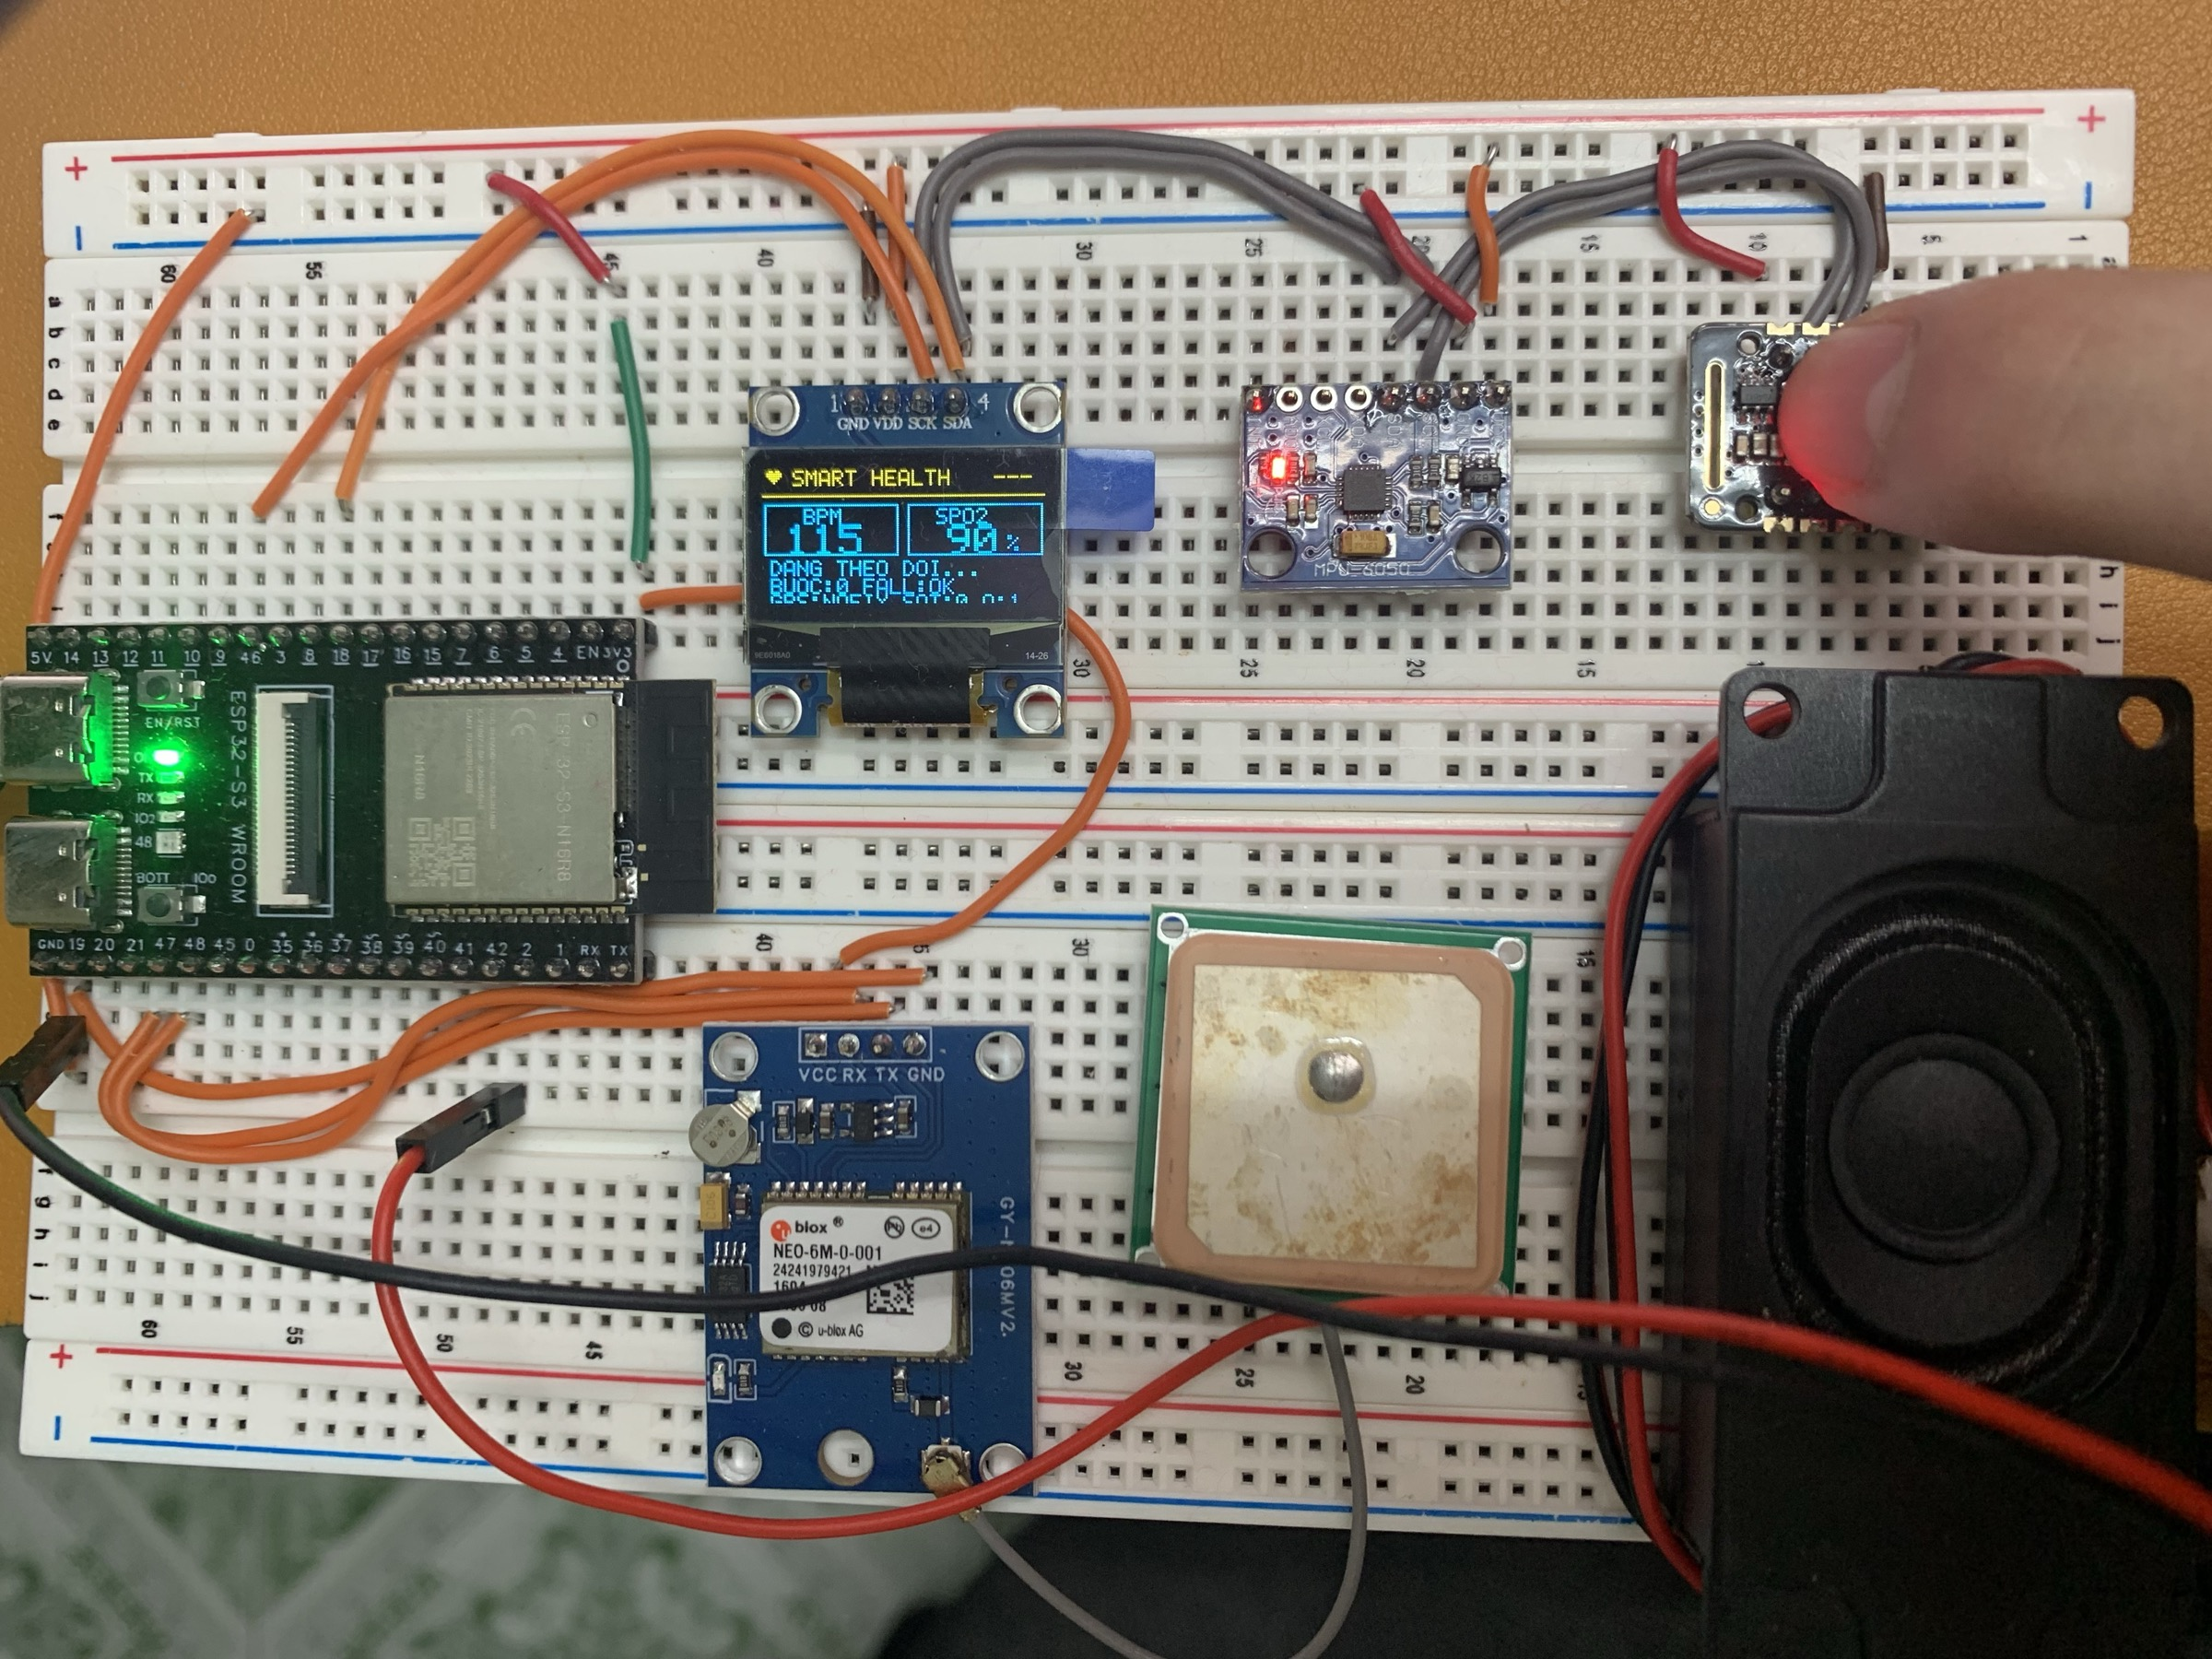
\includegraphics[width=0.96\textwidth,height=10.2cm,keepaspectratio]{assets/product/product_breadboard.jpg}
  \caption{Nguyên mẫu thực tế của nhóm lắp trên breadboard gồm ESP32-S3, OLED, MAX30102, IMU, GPS và buzzer. OLED đang nhận dữ liệu từ firmware tại thời điểm chụp; các số hiển thị trong ảnh chỉ minh họa trạng thái hoạt động, không được dùng làm số liệu hiệu chuẩn y tế. Ảnh do nhóm chụp.}
  \label{fig:working-breadboard-prototype}
\end{figure}

Hình~\ref{fig:working-breadboard-prototype} xác nhận chuỗi phần cứng đã được lắp và chạy đồng thời trên một nguyên mẫu thống nhất, thay vì chỉ kiểm tra từng mô-đun riêng lẻ. Đây là cấu hình được sử dụng để kiểm tra hiển thị OLED, tín hiệu PPG, dữ liệu chuyển động, luồng GPS và cảnh báo âm thanh.

\section{Thiết kế phần mềm}

\subsection{Tổ chức chương trình}

Theo yêu cầu của đồ án, chương trình chỉ dùng các thành phần có sẵn trong ESP32 Arduino Core như \Code{Wire}, UART phần cứng và \Code{millis()}. Các phần được cài đặt trong sketch gồm:

\begin{itemize}
  \item chuỗi lệnh khởi tạo SSD1306, framebuffer, font 5x7 và đồ họa;
  \item cấu hình thanh ghi, đọc FIFO và xử lý tín hiệu MAX30102;
  \item đọc thanh ghi IMU và máy trạng thái phát hiện té ngã;
  \item lọc gia tốc và xác định chuỗi bước đi;
  \item bộ đệm dòng, checksum, tách trường và đổi tọa độ NMEA;
  \item Wi-Fi Access Point, phản hồi DNS captive portal, bộ phân tích/định tuyến HTTP, API JSON và dashboard responsive do nhóm tự viết;
  \item bộ lập lịch theo thời gian và cơ chế phát hiện lại thiết bị.
\end{itemize}

\small
\noindent\begin{tabularx}{\textwidth}{L{3.6cm} L{3.1cm} Y}
\toprule
\textbf{Tệp tiêu đề} & \textbf{Nguồn} & \textbf{Mục đích}\\
\midrule
\Code{Arduino.h} & ESP32 Arduino Core & GPIO, thời gian, LEDC và hàm nền tảng\\
\Code{Wire.h} & ESP32 Arduino Core & Chỉ thực hiện giao tiếp I2C được giảng viên cho phép\\
\Code{HardwareSerial.h} & ESP32 Arduino Core & Nhận byte UART từ GPS\\
\Code{WiFi.h} & ESP32 Arduino Core & Điều khiển radio, Access Point và socket TCP\\
\Code{WiFiUdp.h} & ESP32 Arduino Core & Truyền/nhận datagram UDP mức thấp\\
\Code{math.h} & Thư viện chuẩn C/C++ & Căn bậc hai, trị tuyệt đối\\
\bottomrule
\end{tabularx}
\normalsize

Sketch không dùng Adafruit SSD1306/GFX, SparkFun MAX3010x, TinyGPS++, thư viện MPU, WebServer, DNSServer hay thư viện xử lý tín hiệu. Driver cảm biến, thuật toán, parser NMEA, parser/router HTTP, JSON và phản hồi DNS đều nằm trong mã nguồn của nhóm. \Code{WiFi.h} và \Code{WiFiUdp.h} chỉ là lớp phần cứng/socket bắt buộc thuộc ESP32 Arduino Core.

\subsection{Luồng vòng lặp chính}

Ở mỗi vòng lặp, chương trình xử lý nhanh DNS/HTTP đang chờ, đọc hết byte GPS và rút FIFO PPG. Theo các mốc thời gian riêng, chương trình cập nhật IMU, máy trạng thái té ngã, OLED và nhật ký. Không có trì hoãn dài nên các nguồn dữ liệu tốc độ khác nhau và dashboard vẫn hoạt động đồng thời.

\Needspace{0.38\textheight}
\begin{figure}[htbp]
\centering
\begin{tikzpicture}[
  node distance=6mm and 13mm,
  process/.style={draw=black,rounded corners=1mm,fill=gray!7,minimum width=46mm,minimum height=10mm,align=center,font=\small},
  decision/.style={draw=black,diamond,aspect=2.4,fill=gray!14,inner sep=1.3mm,align=center,font=\small},
  flow/.style={-{Latex[length=2.2mm]},thick,color=black},
  label/.style={font=\scriptsize,fill=white,inner sep=1pt}
]
\node[process] (start) {Bắt đầu một vòng \Code{loop()}};
\node[process,below=of start] (read) {Xử lý DNS/HTTP đang chờ\\Đọc GPS và rút FIFO PPG};
\node[decision,below=of read] (due) {Đến mốc thời gian\\của tác vụ?};
\node[process,below=of due] (tasks) {Cập nhật IMU, phát hiện té ngã\\OLED, buzzer và nhật ký};
\node[process,right=of due] (recover) {Kiểm tra trạng thái\\và phát hiện lại thiết bị};
\draw[flow] (start) -- (read);
\draw[flow] (read) -- (due);
\draw[flow] (due) -- node[label,left]{Có} (tasks);
\draw[flow] (due) -- node[label,above]{Không} (recover);
\draw[flow] (tasks.east) -| (recover.south);
\draw[flow] (recover.north) |- (start.east);
\end{tikzpicture}
\caption{Sơ đồ khối luồng xử lý không chặn trong vòng lặp chính.}
\label{fig:main-loop-flow}
\end{figure}

\subsection{Giao diện OLED}

Màn hình chính ưu tiên BPM và SpO$_2$ bằng ký tự cỡ lớn. Các hàng dưới hiển thị hướng dẫn đo, số bước, trạng thái té ngã, GPS, số vệ tinh/gia tốc hoặc tọa độ luân phiên. Khi có té ngã, toàn màn hình chuyển sang cảnh báo khẩn; nếu GPS vừa mất fix, màn hình dùng tọa độ hợp lệ gần nhất và ký hiệu \Code{L-LAT}/\Code{L-LON}. Các số chân đấu nối không xuất hiện trên giao diện người dùng.

\subsection{Giao diện web qua Wi-Fi}

ESP32-S3 tạo Access Point \Code{health-monitor} với mật khẩu \Code{99999999}. Sau khi kết nối, người dùng mở \path{http://192.168.4.1}. Tài nguyên HTML/CSS/JavaScript nằm trong flash và không dùng CDN. API tại \path{/api/status} trả BPM, SpO$_2$, chất lượng PPG, dữ liệu thô, số bước, trạng thái té ngã, gia tốc, trạng thái từng mô-đun, GPS, vệ tinh, tọa độ, uptime và số máy khách.

Hai endpoint POST cho phép đặt lại số bước và hủy cảnh báo. Dashboard chỉ hiện số sức khỏe khi cờ hợp lệ tương ứng là đúng; liên kết bản đồ chỉ được mở khi hệ thống đã từng nhận tọa độ hợp lệ.

\begin{figure}[htbp]
  \centering
  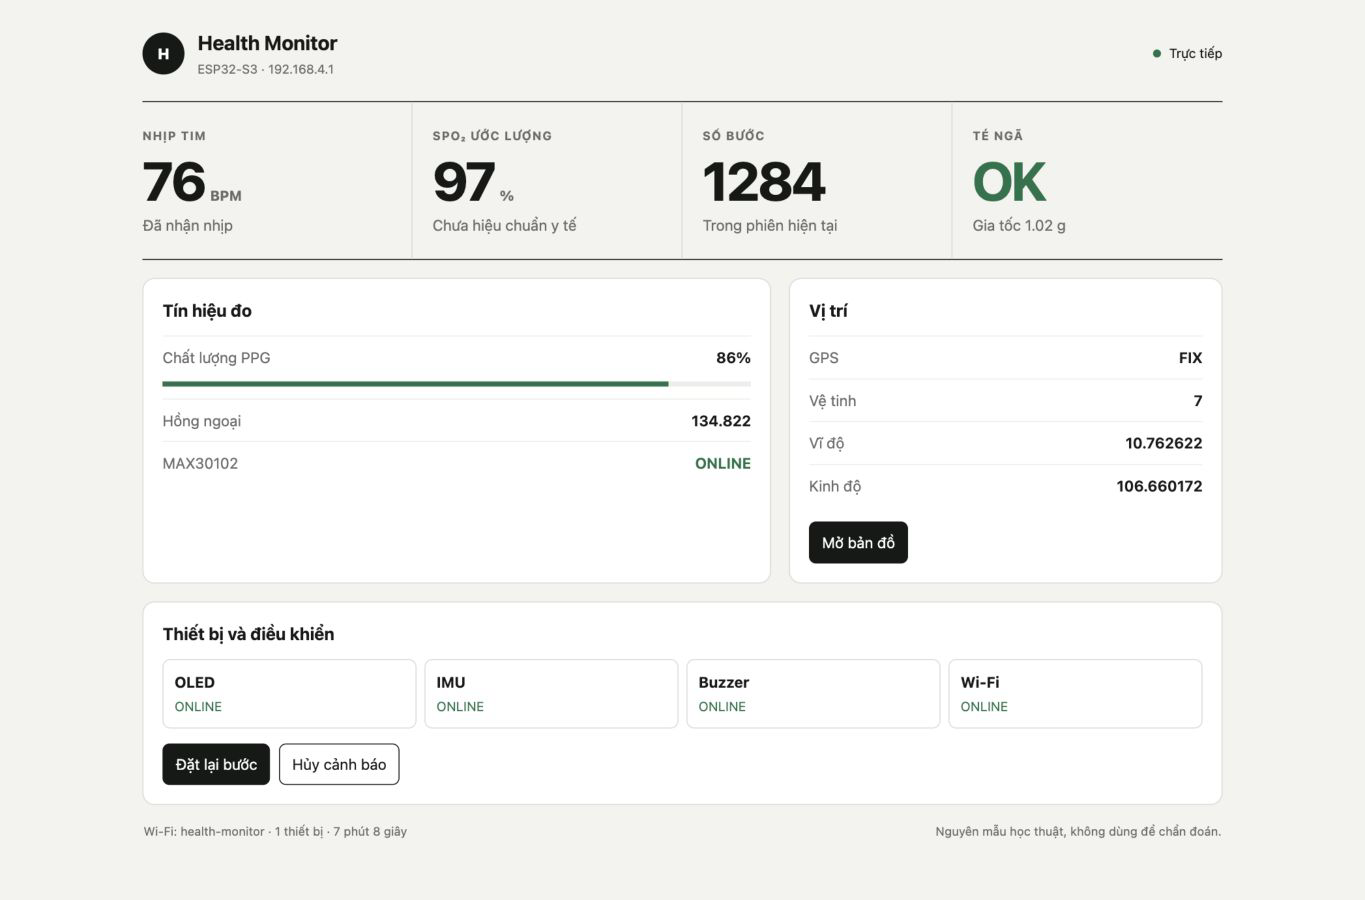
\includegraphics[width=0.98\textwidth,height=8.6cm,keepaspectratio]{assets/web/dashboard_preview.png}
  \caption{Dashboard web tinh gọn được render với dữ liệu minh họa để kiểm tra bố cục. Khi chạy trên ESP32-S3, trang lấy dữ liệu thực từ API JSON mỗi 0,25 giây.}
  \label{fig:web-dashboard}
\end{figure}

\section{Thuật toán các mô-đun}

\subsection{\texorpdfstring{Nhịp tim và SpO$_2$}{Nhịp tim và SpO2}}

MAX30102 cung cấp hai kênh quang RED/IR ở 100 Hz. Trong 0,35 giây đầu, bộ lọc bám nhanh theo mức DC để xung đặt tay không làm ngưỡng nhịp tăng sai. Sau đó, hai cạnh trái dấu tạo BPM sơ bộ từ nửa chu kỳ; cạnh cùng cực tính kế tiếp xác nhận RR đầy đủ và thay số sơ bộ. Nếu không có RR xác nhận trong 1,8 giây, số sơ bộ tự bị hủy. SpO$_2$ dùng tỷ lệ giữa AC/DC trong cửa sổ 64 mẫu, được xét độc lập với BPM và có thể xuất sau khoảng một giây nếu tín hiệu quang đạt điều kiện.

Ngưỡng nhận tay là IR lớn hơn 10.000; sau khi đã nhận, ngưỡng nhả giảm còn 7.000 để tạo vùng trễ. Hụt tín hiệu dưới 450 ms chưa xóa số đo, nhưng nếu tay quay lại sau ít nhất 180 ms thì cạnh, cực tính và RR cũ bị xóa để bắt đầu phiên mới. Khi đặt lại tay hoặc bộ dò chưa tìm được BPM sau 3,5 giây, vòng lặp yêu cầu khởi tạo lại MAX30102 và FIFO; vì vậy việc bắt lại không phụ thuộc thao tác mở Serial Monitor.

\subsection{Phát hiện té ngã}

Độ lớn gia tốc ba trục được đưa qua chuỗi trạng thái NORMAL, FREEFALL, IMPACT và ALERT. Cảnh báo chỉ sinh ra nếu ba hiện tượng rơi tự do, va đập và ít chuyển động xuất hiện đúng thứ tự trong các cửa sổ thời gian cho phép.

\subsection{Đếm bước}

Thành phần gia tốc chậm được dùng làm đường nền. Chương trình đếm các đỉnh chuyển động có khoảng cách 280--1.800 ms và chỉ bắt đầu cộng khi có hai đỉnh liên tiếp. Số bước được giữ trong RAM cho đến khi thiết bị khởi động lại.

\subsection{GPS}

GPS dùng UART1 ở 9.600 baud và được đọc hết byte đang chờ trong mỗi vòng lặp. Bộ đệm tự gom câu từ ký tự ``\$'' đến cuối dòng, kiểm tra checksum XOR rồi mới tách tối đa 16 trường. GGA cung cấp chất lượng fix, số vệ tinh và tọa độ; RMC chỉ được nhận khi trạng thái bằng A. Tọa độ ddmm.mmmm/dddmm.mmmm được đổi sang độ thập phân, kiểm tra bán cầu và giới hạn vĩ/kinh độ trước khi lưu. Hệ thống tách WAIT, LOST, NOFIX và FIX theo bộ đếm byte cùng thời điểm nhận dữ liệu/fix gần nhất để tránh hiểu nhầm chưa bắt vệ tinh là lỗi dây.

\section{Các đoạn mã quyết định}

Các đoạn dưới đây được trích từ sketch nộp kèm. Chúng thể hiện những điều kiện trực tiếp quyết định đầu ra của hệ thống; mã đầy đủ còn chứa phần khởi tạo, vẽ giao diện và nhật ký kiểm tra.

\subsection{Phân biệt FIFO rỗng với lỗi MAX30102}

\Needspace{0.28\textheight}
\begin{lstlisting}[style=firmware,caption={Không dùng dữ liệu PPG cũ khi cảm biến mất kết nối}]
(*@\VNCodeComment{Đọc một mẫu từ FIFO MAX30102 và lưu loại kết quả trả về.}@*)
int8_t result = MAX30102_ReadFIFO();
(*@\VNCodeComment{Thoát vòng đọc khi FIFO hiện không có mẫu mới; đây không phải lỗi cảm biến.}@*)
if (result == FIFO_NO_DATA) break;
(*@\VNCodeComment{Đi vào nhánh xử lý riêng khi giao dịch I2C với MAX30102 thất bại.}@*)
if (result == FIFO_BUS_ERROR) {
(*@\VNCodeComment{Đánh dấu cảm biến quang đang mất kết nối để cơ chế phục hồi có thể khởi tạo lại.}@*)
  maxOK = false;
(*@\VNCodeComment{Xóa BPM, SpO2 và trạng thái bộ lọc để không giữ số đo của phiên cũ.}@*)
  PPG_ResetMetrics();
(*@\VNCodeComment{Đặt cả hai mẫu quang thô về 0, tránh giao diện hiểu dữ liệu cũ là mẫu mới.}@*)
  ppg.redRaw = ppg.irRaw = 0;
(*@\VNCodeComment{Dừng vòng đọc FIFO ngay sau lỗi bus.}@*)
  break;
(*@\VNCodeComment{Kết thúc nhánh xử lý lỗi giao tiếp.}@*)
}
\end{lstlisting}

\subsection{Xác nhận BPM trước khi hiển thị}

\Needspace{0.24\textheight}
\begin{lstlisting}[style=firmware,caption={Khoảng RR hợp lệ đầu tiên tạo BPM ban đầu}]
(*@\VNCodeComment{Dùng ngay RR đầy đủ nếu giá trị trước là sơ bộ, chưa hợp lệ hoặc bộ dò vừa bắt đầu lại.}@*)
if (ppg.heartRateProvisional || !ppg.heartRateValid ||
    state.replaceBpmOnNextInterval) {
  ppg.bpm = instantBPM;
  ppg.heartRateValid = true;
  ppg.heartRateProvisional = false;
  state.replaceBpmOnNextInterval = false;
(*@\VNCodeComment{Chỉ làm mượt nhịp kế tiếp khi lệch không quá 18 BPM so với số đang hiển thị.}@*)
} else if (fabsf(instantBPM - ppg.bpm) <= 18.0f) {
(*@\VNCodeComment{Giữ 90\% giá trị cũ và nhận 10\% giá trị mới để OLED ổn định hơn khi ngón tay rung nhẹ.}@*)
  ppg.bpm = 0.90f * ppg.bpm + 0.10f * instantBPM;
}
\end{lstlisting}

\Needspace{0.42\textheight}
\subsection{Điều kiện bước chân và té ngã}
\begin{lstlisting}[style=firmware,caption={Ngưỡng động học dùng cho hai chức năng IMU}]
(*@\VNCodeComment{Chỉ xét một bước khi đã thấy đáy âm và tín hiệu động vượt ngưỡng dương 0,11 g.}@*)
if (peakArmed && dynamicFiltered > 0.11f &&
(*@\VNCodeComment{Yêu cầu cách đỉnh trước hơn 280 ms và tổng gia tốc nhỏ hơn 1,8 g để loại rung hoặc va đập.}@*)
    now - lastPeakMs > 280 && totalG < 1.8f) {
(*@\VNCodeComment{Tính thời gian giữa hai đỉnh; khi chưa có đỉnh trước thì trả về 0.}@*)
  uint32_t interval = lastPeakMs == 0 ? 0 : now - lastPeakMs;
(*@\VNCodeComment{Xác nhận chu kỳ nằm trong miền 280--1.800 ms của một nhịp bước hợp lý.}@*)
  if (interval >= 280 && interval <= 1800) {
(*@\VNCodeComment{Kiểm tra chuỗi đi bộ đã được xác nhận hay mới bắt đầu.}@*)
    if (walkingSequence) {
(*@\VNCodeComment{Nếu chuỗi đang hợp lệ, cộng thêm đúng một bước cho đỉnh mới.}@*)
      stepCount++;
(*@\VNCodeComment{Đi vào nhánh khởi tạo khi vừa có cặp đỉnh hợp lệ đầu tiên.}@*)
    } else {
(*@\VNCodeComment{Cộng hai bước để tính cả đỉnh đầu tiên từng được giữ lại để xác nhận chuỗi.}@*)
      stepCount += 2;
(*@\VNCodeComment{Đánh dấu các đỉnh tiếp theo thuộc cùng một chuỗi đi bộ.}@*)
      walkingSequence = true;
(*@\VNCodeComment{Kết thúc lựa chọn cách cập nhật bộ đếm bước.}@*)
    }
(*@\VNCodeComment{Kết thúc điều kiện chu kỳ bước hợp lệ.}@*)
  }
(*@\VNCodeComment{Kết thúc điều kiện xác nhận đỉnh dương.}@*)
}
(*@\VNCodeComment{Máy trạng thái dưới đây giữ đủ chuỗi NORMAL--FREE\_FALL--IMPACT--ALERT như firmware.}@*)
switch (fallState) {
  case FALL_NORMAL:
    if (accelerationG < 0.45f) {
      if (lowGStartMs == 0) lowGStartMs = now;
      if (now - lowGStartMs >= 120) {
        fallState = FALL_FREE_FALL;
        fallStateMs = now;
      }
    } else {
      lowGStartMs = 0;
    }
(*@\VNCodeComment{Va đập trực tiếp trên 2,8 g cũng có thể mở ngay giai đoạn kiểm tra bất động.}@*)
    if (accelerationG > 2.8f) {
      fallState = FALL_IMPACT;
      fallStateMs = now;
    }
    break;

  case FALL_FREE_FALL:
(*@\VNCodeComment{Sau rơi tự do phải có va đập trên 2,2 g trong 1.200 ms; quá hạn thì hủy chuỗi.}@*)
    if (accelerationG > 2.2f) {
      fallState = FALL_IMPACT;
      fallStateMs = now;
    } else if (now - fallStateMs > 1200) {
      fallState = FALL_NORMAL;
      lowGStartMs = 0;
    }
    break;

  case FALL_IMPACT:
(*@\VNCodeComment{Sau va đập, chỉ cảnh báo khi bất động hơn 1.800 ms và tổng gia tốc trở về gần 1 g.}@*)
    if (now - fallStateMs > 1800 && motionLevel < 0.08f &&
        accelerationG > 0.72f && accelerationG < 1.28f) {
      fallState = FALL_ALERT;
      fallStateMs = now;
      Serial.println(
        "[ALERT] PHAT HIEN TE NGA - CAN KIEM TRA NGUOI DUNG");
    } else if (now - fallStateMs > 5000) {
      fallState = FALL_NORMAL;
    }
    break;

  case FALL_ALERT:
(*@\VNCodeComment{Giữ cảnh báo để OLED, buzzer và dashboard tiếp tục phản ánh cùng một trạng thái.}@*)
    break;
}
\end{lstlisting}

\Needspace{0.28\textheight}
\subsection{Loại câu NMEA sai checksum}
\begin{lstlisting}[style=firmware,caption={Hàm kiểm tra đầy đủ checksum NMEA}]
(*@\VNCodeComment{Đổi một chữ số hexadecimal sang giá trị 0--15; ký tự lạ trả -1.}@*)
int8_t NMEA_HexNibble(char c) {
  if (c >= '0' && c <= '9') return c - '0';
  if (c >= 'A' && c <= 'F') return c - 'A' + 10;
  if (c >= 'a' && c <= 'f') return c - 'a' + 10;
  return -1;
}

(*@\VNCodeComment{Chỉ nhận câu bắt đầu bằng đô-la, có dấu sao và đủ hai chữ số checksum.}@*)
bool NMEA_ChecksumOK(const char *sentence) {
  if (!sentence || sentence[0] != '$') return false;
  const char *star = strchr(sentence, '*');
  if (!star || strlen(star) < 3) return false;
  int8_t high = NMEA_HexNibble(star[1]);
  int8_t low = NMEA_HexNibble(star[2]);
  if (high < 0 || low < 0) return false;
(*@\VNCodeComment{XOR toàn bộ phần thân giữa ký tự đô-la và dấu sao.}@*)
  uint8_t checksum = 0;
  for (const char *p = sentence + 1; p < star; p++) {
    checksum ^= (uint8_t)*p;
  }
(*@\VNCodeComment{Ghép hai nửa byte và so sánh với checksum tự tính.}@*)
  uint8_t expected = (uint8_t)((high << 4) | low);
  return checksum == expected;
}
\end{lstlisting}

\subsection{Đổi và kiểm tra tọa độ}
\begin{lstlisting}[style=firmware,caption={Đổi tọa độ NMEA và chỉ lưu giá trị hợp lệ}]
(*@\VNCodeComment{Tách phần độ và phút, sau đó đổi sang độ thập phân.}@*)
double NMEA_ToDegrees(const char *value, char hemisphere) {
  if (!value || !*value) return 0.0;
  double raw = atof(value);
  int degrees = (int)(raw / 100.0);
  double minutes = raw - degrees * 100.0;
  double result = degrees + minutes / 60.0;
(*@\VNCodeComment{Bán cầu Nam hoặc Tây làm kết quả mang dấu âm.}@*)
  if (hemisphere == 'S' || hemisphere == 'W') result = -result;
  return result;
}

(*@\VNCodeComment{Loại trường rỗng, ký hiệu bán cầu sai và tọa độ vượt miền địa lý.}@*)
bool GPS_StorePosition(const char *latitude, char northSouth,
                       const char *longitude, char eastWest) {
  if (!latitude || !longitude || !latitude[0] || !longitude[0]) return false;
  if (northSouth != 'N' && northSouth != 'S') return false;
  if (eastWest != 'E' && eastWest != 'W') return false;
  double parsedLatitude = NMEA_ToDegrees(latitude, northSouth);
  double parsedLongitude = NMEA_ToDegrees(longitude, eastWest);
  if (fabs(parsedLatitude) > 90.0 ||
      fabs(parsedLongitude) > 180.0) return false;
(*@\VNCodeComment{Lưu tọa độ, hai cờ vị trí và thời điểm fix mới nhất cho mọi giao diện.}@*)
  gpsLatitude = parsedLatitude;
  gpsLongitude = parsedLongitude;
  gpsFix = true;
  gpsPositionKnown = true;
  lastGPSFixMs = millis();
  return true;
}
\end{lstlisting}

\subsection{Tách GGA và RMC}
\begin{lstlisting}[style=firmware,caption={Parser câu GGA/RMC sau khi checksum hợp lệ}]
(*@\VNCodeComment{Không xử lý tiếp nếu câu NMEA sai checksum.}@*)
void GPS_ParseSentence(const char *sentence) {
  if (!NMEA_ChecksumOK(sentence)) return;
  char copy[96];
  strncpy(copy, sentence, sizeof(copy));
  copy[sizeof(copy) - 1] = '\0';
  char *star = strchr(copy, '*');
  if (star) *star = '\0';

(*@\VNCodeComment{Tự tách tối đa 16 trường bằng dấu phẩy, không dùng thư viện parser GPS.}@*)
  char *fields[16] = {nullptr};
  uint8_t count = 1;
  fields[0] = copy;
  for (char *p = copy; *p && count < 16; p++) {
    if (*p == ',') {
      *p = '\0';
      fields[count++] = p + 1;
    }
  }
  if (count == 0) return;
  bool isGGA = strstr(fields[0], "GGA") != nullptr;
  bool isRMC = strstr(fields[0], "RMC") != nullptr;

(*@\VNCodeComment{GGA cập nhật số vệ tinh; quality bằng 0 hoặc tọa độ sai làm mất fix.}@*)
  if (isGGA && count > 7) {
    uint8_t quality = (uint8_t)atoi(fields[6]);
    gpsSatellites = (uint8_t)atoi(fields[7]);
    if (quality == 0 ||
        !GPS_StorePosition(fields[2], fields[3][0],
                           fields[4], fields[5][0])) {
      gpsFix = false;
    }
(*@\VNCodeComment{RMC chỉ hợp lệ khi trường trạng thái bằng A và vị trí qua kiểm tra.}@*)
  } else if (isRMC && count > 6) {
    if (fields[2][0] != 'A' ||
        !GPS_StorePosition(fields[3], fields[4][0],
                           fields[5], fields[6][0])) {
      gpsFix = false;
    }
  }
}
\end{lstlisting}

\subsection{Thu UART và phân loại trạng thái GPS}
\begin{lstlisting}[style=firmware,caption={Gom dòng NMEA và trả WAIT/LOST/NOFIX/FIX}]
(*@\VNCodeComment{Đọc hết byte chờ, cập nhật bộ đếm và thời điểm nhận gần nhất.}@*)
void GPS_Poll() {
  while (gpsSerial.available() > 0) {
    char c = (char)gpsSerial.read();
    gpsByteCount++;
    lastGPSByteMs = millis();
(*@\VNCodeComment{Đô-la mở câu mới; xuống dòng kết thúc câu và gọi parser.}@*)
    if (c == '$') {
      gpsWorkingLength = 0;
      gpsWorking[gpsWorkingLength++] = c;
    } else if (c == '\n') {
      if (gpsWorkingLength > 0) {
        gpsWorking[gpsWorkingLength] = '\0';
        GPS_ParseSentence(gpsWorking);
        gpsWorkingLength = 0;
      }
(*@\VNCodeComment{Bỏ CR và chống tràn bộ đệm 96 byte khi nối phần thân câu.}@*)
    } else if (c != '\r' && gpsWorkingLength > 0 &&
               gpsWorkingLength < sizeof(gpsWorking) - 1) {
      gpsWorking[gpsWorkingLength++] = c;
    }
  }
}

(*@\VNCodeComment{Phân biệt chưa nhận byte, mất UART, fix còn mới và đang nhận nhưng chưa fix.}@*)
const char *GPS_StatusText() {
  if (gpsByteCount == 0) return "WAIT";
  if (millis() - lastGPSByteMs > 3000) return "LOST";
  if (gpsFix && millis() - lastGPSFixMs < 10000) return "FIX";
  return "NOFIX";
}
\end{lstlisting}

\section{Phân công thực hiện}

\begin{tabularx}{\textwidth}{L{3.4cm} Y C{2cm}}
\toprule
\textbf{Thành viên} & \textbf{Phần việc chính} & \textbf{Tỷ lệ}\\
\midrule
Phạm Hùng Tiến & Tích hợp, I2C/OLED, Wi-Fi AP, HTTP/DNS tự viết, khung dashboard, lịch chạy và kiểm thử tổng & 33,4\%\\
Hồ Sĩ Phú & MAX30102/PPG, BPM, SpO$_2$, chất lượng và hợp đồng dữ liệu PPG cho web & 33,3\%\\
Quách Gia Thịnh & IMU/GPS, té ngã, dữ liệu vị trí/chuyển động và thao tác điều khiển web & 33,3\%\\
\bottomrule
\end{tabularx}

Các phần việc được ghép và kiểm tra chung trên cùng một phiên bản chương trình.

\section{Kiểm thử và kết quả}

\begin{longtable}{L{4.2cm} L{5.8cm} L{3.1cm}}
\toprule
\textbf{Phép thử} & \textbf{Kết quả đo/quan sát} & \textbf{Đánh giá}\\
\midrule
\endfirsthead
\toprule
\textbf{Phép thử} & \textbf{Kết quả đo/quan sát} & \textbf{Đánh giá}\\
\midrule
\endhead
Quét I2C & Phát hiện 0x3C, 0x57, 0x68 & \OK\\
Định danh IMU & WHO\_AM\_I = 0x74 & \OK\\
Gia tốc nghỉ & 1,07--1,08$g$ & \OK\\
Đếm bước khi đặt yên & Bộ đếm giữ nguyên 0 & \OK\\
Đếm bước mô phỏng & 20 chu kỳ tổng hợp cho 20 bước; nhiễu nhỏ/rung đơn cho 0 & \OK\\
Đếm bước khi đi bộ & Chưa có chuỗi đối chứng đủ dài để tính sai số & \NeedTest\\
MAX30102 rời tay & IR 330--400, kết quả ở WAIT & \OK\\
MAX30102 đặt tay & IR 132.000--137.000 & \OK\\
Nhịp tim & BPM quan sát khoảng 72--83 qua các lần thử & \OK\\
Thời gian PPG tổng hợp & BPM sơ bộ có thể dưới 1 giây, xác nhận theo RR; SpO$_2$ từ khoảng 1 giây khi tín hiệu đạt chuẩn & \OK\\
Dạng sóng PPG đảo & Bộ dò tự nhận cực tính dương/âm và vẫn khôi phục đúng BPM & \OK\\
SpO$_2$ nguyên mẫu & Khoảng 90--96\% trong các lần thử gần nhất & \Pending\\
Luồng GPS & Hơn 7.000 byte NMEA; không mất UART & \OK\\
GPS có vị trí & FIX, 4 vệ tinh ở lần chạy cuối, có vĩ/kinh độ & \OK\\
Buzzer/LEDC & Kênh PWM khởi tạo thành công; chưa đo mức âm thực tế & \Implemented\\
Wi-Fi Access Point & SSID \Code{health-monitor}; IP 192.168.4.1; dashboard và API phản hồi & \Implemented\\
Dashboard responsive & Hiển thị đủ PPG, bước, té ngã, thiết bị, GPS và trạng thái hệ thống & \OK\\
Điều khiển web & Đặt lại bước và hủy cảnh báo trả JSON thành công & \OK\\
Té ngã mô phỏng & Chuỗi đầy đủ vào ALERT; chuỗi thiếu va đập về NORMAL & \OK\\
Té ngã thực tế & Chưa thử ngã người thật; chỉ mới kiểm tra logic và ngưỡng trên mô hình & \NeedTest\\
Biên dịch & 969.218 byte flash (30\%), RAM 49.972 byte (15\%) & \OK\\
Nạp phần cứng & Xác minh hash, hard reset thành công & \OK\\
\bottomrule
\end{longtable}

Các ca mô phỏng được tái lập bằng tệp \path{tests/algorithm_selfcheck.py}, chỉ dùng thư viện chuẩn Python và giữ nguyên hệ số/ngưỡng của firmware. Chúng chứng minh luồng quyết định chạy nhất quán nhưng không được dùng để thay thế số liệu đi bộ hoặc té ngã trên người thật.

Ảnh nguyên mẫu tại Hình~\ref{fig:working-breadboard-prototype} bổ sung bằng chứng trực quan cho phép thử tích hợp: ESP32-S3, màn hình, cảm biến quang, IMU, GPS và buzzer cùng hiện diện trên breadboard; OLED hiển thị dữ liệu trong khi người dùng đặt ngón tay lên MAX30102.

\section{Đánh giá rủi ro và giới hạn}

\begin{itemize}
  \item SpO$_2$ chưa được hiệu chuẩn bằng thiết bị y tế tham chiếu, vì vậy chỉ mang tính học thuật.
  \item Chuyển động ngón tay, ánh sáng ngoài và lực ép làm giảm độ tin cậy PPG.
  \item GPS trong nhà có thể ở NOFIX hoặc số vệ tinh thấp; cần thử ngoài trời.
  \item Dashboard hiện dùng mạng cục bộ với một mật khẩu dùng chung; chưa có tài khoản, HTTPS hoặc phân quyền thao tác.
  \item Ngưỡng té ngã cần được đánh giá trên nhiều tư thế và đối tượng nhưng phải dùng đệm, dây giữ và quy trình an toàn.
  \item Nguyên mẫu chưa có quản lý pin, vỏ đeo, động cơ rung, nút hủy cảnh báo và kênh gửi cảnh báo từ xa.
\end{itemize}

\section{Hướng phát triển}

Nhóm đề xuất bổ sung nút SOS/hủy vật lý và động cơ rung; hiệu chuẩn SpO$_2$; ghi lịch sử đo; thêm xác thực web; dùng BLE/Wi-Fi STA/LTE để gửi cảnh báo ra ngoài mạng cục bộ; tối ưu tiêu thụ điện; thiết kế PCB và vỏ đeo. Đối với té ngã, ngưỡng cố định có thể được thay bằng mô hình thích nghi sau khi có bộ dữ liệu thử nghiệm đủ lớn.

\section{Kết luận}

Mô hình đã đọc cảm biến, hiển thị số đo trên OLED và web, nhận vị trí GPS, đồng thời điều khiển màn hình/loa khi máy trạng thái té ngã được kích hoạt. Kiến trúc không chặn cho phép cảm biến và dịch vụ HTTP/DNS tự viết dùng chung ESP32-S3. Trước khi sử dụng thực tế, sản phẩm cần được hiệu chuẩn, thử nghiệm an toàn và hoàn thiện bảo mật, nguồn, vỏ đeo cùng kênh truyền tin từ xa.

\section*{Tài liệu tham khảo}
\addcontentsline{toc}{section}{Tài liệu tham khảo}

\begin{itemize}
  \item Espressif Systems, \href{https://docs.espressif.com/projects/esp-idf/en/stable/esp32s3/hw-reference/index.html}{ESP32-S3 Hardware Reference}.
  \item Espressif Systems, \href{https://github.com/espressif/arduino-esp32}{Arduino Core for ESP32} và mã nguồn \Code{Wire} đi kèm.
  \item Analog Devices, \href{https://www.analog.com/media/en/technical-documentation/data-sheets/MAX30102.pdf}{MAX30102 Datasheet, Revision 1}.
  \item Analog Devices, \href{https://www.analog.com/en/resources/technical-articles/guidelines-for-spo2-measurement--maxim-integrated.html}{hướng dẫn hiệu chuẩn phép đo SpO$_2$}.
  \item Freenove, \href{https://store.freenove.com/products/fnk0085}{ESP32-S3-WROOM Camera Board, dòng FNK0085}; nguồn ảnh bo điều khiển.
  \item Waveshare, \href{https://www.waveshare.com/0.96inch-OLED-A.htm}{OLED SSD1306 0,96 inch 128x64} và \href{https://www.waveshare.com/uart-gps-neo-6m.htm}{mô-đun GPS UART NEO-6M}; nguồn ảnh tham chiếu.
  \item DFRobot, \href{https://wiki.dfrobot.com/sen0344/docs/19237}{Fermion MAX30102 V1.0}; nguồn ảnh bo breakout tham chiếu.
  \item TDK InvenSense, \href{https://invensense.tdk.com/wp-content/uploads/2015/02/MPU-6000-Register-Map.pdf}{MPU-6000/MPU-6050 Register Map, Revision 4.2}; dùng để đối chiếu nhóm thanh ghi gia tốc tương thích.
  \item Solomon Systech, \href{https://www.solomon-systech.com/product-category/oled-display}{danh mục bộ điều khiển OLED SSD1306 128x64}.
\end{itemize}

\end{document}
